\documentclass{llncs}
\usepackage{llncsdoc}
\usepackage[english]{babel}
\usepackage[utf8x]{inputenc}
\usepackage{graphicx}
\usepackage{pmboxdraw}
\usepackage{color}
\definecolor{darkgray}{rgb}{0.41, 0.41, 0.41}
\definecolor{green}{rgb}{0.0, 0.5, 0.0}
\usepackage{listingsutf8}
\lstset{language=Prolog, 
	numbers=left,
	stepnumber=5,
	firstnumber=1,
	numberfirstline=true,
    basicstyle=\linespread{0.8}\ttfamily,
    keywordstyle=\color{blue}\ttfamily,
	showstringspaces=false,
    stringstyle=\color{red}\ttfamily,
    commentstyle=\color{green}\ttfamily,
	identifierstyle=\color{darkgray}\ttfamily,
    morecomment=[l][\color{magenta}]{\#},
	tabsize=1,
    breaklines=true,
    extendedchars=true,
	inputencoding=utf8x,
    escapeinside={\%*}{*)},
}
\lstset{literate=%
{↑}{{$\uparrow}$}1
{→}{{$\rightarrow}$}1
{↓}{{$\downarrow}$}1
{←}{{$\rightarrow}$}1
{│}{{$\textSFxi$}}1
{─}{{$\textSFx}$}1
{┌}{{$\textSFi}$}1
{┬}{{$\textSFvi}$}1
{┐}{{$\textSFiii}$}1
{├}{{$\textSFviii}$}1
{┼}{{$\textSFv}$}1
{┤}{{$\textSFix}$}1
{└}{{$\textSFii}$}1
{┴}{{$\textSFvii}$}1
{┘}{{$\textSFiv}$}1
}


\begin{document}

\title{Solving the Puzzle Magnets with Constraint Logic Programming}
\author{\^Angela Cardoso \and Nuno Valente}
\institute{FEUP-PLOG, Turma 3MIEIC02, Grupo Magnets\_2.}
\maketitle


\begin{abstract}
	
	This project was developed as part of the coursework for the subject of Logic Programming at the Faculty of Engineering of the University of Porto. In order to learn logic programming with constraints, we chose the puzzle Magnets to implement in SICStus Prolog. The application obtained is capable of solving a given Magnets puzzle, as long as it is supplied in a specific format, generating random puzzles of the required size and displaying both the puzzle and the solution in a user friendly text format. The efficiency of the solution we obtained depends, of course, on the size of the puzzle, but more so on its degree of difficulty. One can easily obtain puzzles where the constraints do not allow for immediate variable reduction, which leads to frequent backtracking and thus long execution times. There is also a lot of symmetry in theses puzzles, which in a straightforward implementation often increments the difficulty of reaching a solution. 
	
\end{abstract}


\section{Introduction}

Constraint logic programming is very useful to solve problems in which one wants to determine a set of variables that must satisfy certain rules. In addition to the the logic programming literals, these programs contain constraints such as~$X \neq Y$. The goal of the program is to determine values for all the variables such that all the clauses and constraints are satisfied. Typically, this kind of programming is used to solve search problems, such as paper-and-pencil puzzles or chess puzzles, and optimization problems, such as scheduling, timetabling, resource allocation, planning, production management or circuit check. By using constraint logic programming one can reduce the development time, as well as obtain efficient, simple and easy to maintain solutions.

To solidify our knowledge of constraint logic programming, we chose to implement the paper-and-pencil puzzle Magnets. In this puzzle, one is given a square grid of dominoes, as well as the number of positive and negative poles for each row and column. Some dominoes are magnetized, having a positive pole and a negative pole, while others are neutral. Also, poles with the same charge repel and are not allowed to touch vertically or horizontally. The objective is identify the positive poles with a $+$ sign, the negative poles with a~$-$ sign and the neutral ones with an~$x$.

The following sections describe the progress of our work on this subject, with details of our implementation and of the results we obtained, including statistics that give some insight to the quality of our solution.

%Descricao dos objetivos e motivacao do trabalho, referencia sucinta ao problema em analise (idealmente, referencia a outros trabalhos sobre o mesmo problema e sua abordagem), e descricao sucinta da estrutura do resto do artigo.


\section{Problem Description} 

Although we managed to find several online implementations or descriptions of the Magnets puzzle, we could not determine its origins. In any case, the rules are quite clear:
\begin{itemize}
	\item for each row and each column the number of positive and negative poles must be as specified;
	\item each charged domino must have a positive and a negative pole;
	\item two positive, or two negative, charged poles must not be vertically or horizontally adjacent.
\end{itemize}
Figure~\ref{example} illustrates these rules, showing a solved magnets puzzle.

\begin{figure}[htbp]
\begin{center}
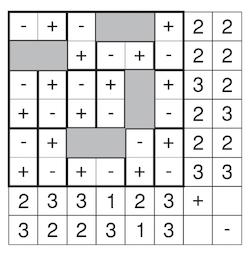
\includegraphics[scale=0.6]{magnets.jpg}
\caption{Example of a Magnets puzzle}
\label{example}
\end{center}
\end{figure}

Our objective is to use constraint logic programming to implement a Magnets puzzle solver. Theoretically, our implementation should be able to handle any such puzzle. However, the exponential nature of such puzzles will certainly impose limitations on any devised implementation. Hence, it is also our intent to obtain an efficient method to solve these puzzles.


\section{Approach}

Even a casual observation of the rules of Magnets gives some clue that this puzzle is suited for constraint logic programming. We shall make this clear in the following sections, where we present a formal description of Magnets as a constraint satisfaction problem (CSP).

\subsection{Decision Variables} 

In any CSP there are variables whose value we aim to determine. For magnets, the decision variables are the half dominoes or poles, that is, each small square in the grid is a decision variable. In order to solve the puzzle, we must obtain the value (positive, negative or neutral) of each of these poles. To better represent these values, and in order to allow for constraint resolution in SICStus Prolog, we used the following conversions:
\begin{itemize}
	\item 1 represents positive poles;
	\item -1 represents negative poles;
	\item 0 represents neutral poles. 
\end{itemize}

Since Magnets puzzles are square grids of a given size~$N$, the number of decision variables is~$N^2$. Each of these variables has 3 possible values, therefore there is a total of $3^{N^2}$ possible solutions to be tested. These variables are organized sequentially in a list from top of the grid to bottom and from left to right.

\subsection{Constraints} 

For each Magnets rule, there is a rigid constraint in our Magnets CSP. The first restriction is on the number of positive and negative poles for each row and column. In order to implement this in SICStus Prolog, we used the combinatorial constraint \verb|global_cardinality|. First we organize our puzzle as a list of lines, then we use \verb|global_cardinality| to force each line to have a specific number of~$1s$,~$0s$ and~$-1s$. Afterwards, the same thing is done for the columns.

The second rule forces each charged domino or magnet to have a positive and a negative pole. This is done with a simple arithmetic constraint. Given our codification of positive, negative and neutral, the sum of both poles of a magnet must be zero. Hence, we use the constraint \verb|#=| to enforce this equality.

Finally, there is a rule on the proximity of same charge poles. Two positive (respectively, negative) poles repel each other, therefore, they cannot be vertically or horizontally adjacent. Again, we check this with an arithmetic constraint. Given two neighbor (vertically or horizontally adjacent) poles, the sum of their cannot be bellow -1 or above 1. Indeed, we can only obtain 2 if there are two positive adjacent poles, and the same thing for -2 and negative poles. Hence, we use the constraints \verb|#>| and \verb|#<| to verify this last rule.

\subsection{Search Strategy} 

In order to attribute values to the variables, SICStus uses the predicate labeling, for which one may provide some options that, depending on the problem at hand, may increase the efficiency of the search for a solution. In our implementation of magnets, these options where mainly chosen through trial and error. In fact, we started by using no options at all (which is the same as using the default options) and then, with a collection of somewhat difficult puzzles, we determined the options with better time performance. 

The first option to consider is variable ordering. That is, which variable should be first consider when Prolog tries to find a possible solution. The default option starts with the leftmost variable, in our case, the first square of the grid. There are several other options that we will not exhaustively mention, because we quickly concluded that they are not suitable for our problem. Besides \verb|leftmost| the ones we tested where:
\begin{itemize}
	\item \verb|first_fail|, which chooses the leftmost variable with the smallest domain;
	\item \verb|occurrence|, which chooses the leftmost variable with the largest number of constraints;
	\item \verb|ffc|, which combines first \verb|first_fail| and \verb|occurrence|.
\end{itemize}
The performance of these options is not always consistent, that is, the better option depends on the specific example. However, in our limited experiments, there seems to be an advantage for \verb|first_fail|, even though sometimes \verb|leftmost| is better. Ordering options including \verb|occurrence| did not perform well in our examples. This is probably due to the fact that the number of restrictions on each variable is more or less the same, with the exception being the extremes of the puzzle, since they have less neighbors. In the end, we opted to use \verb|first_fail|, both because it makes theoretical sense and because there is some limited evidence of its superiority.

The next option is about value selection. Given a variable and a set of possible values for that variable, how should Prolog decide which one to try first. We also made some experiments with these options, but we quickly decided on the best one. Indeed, there are at most three possible values for a Magnets variable:~$-1$,~$0$ and~$1$. For every~$-1$ there is a~$1$, because of the second rule, that is, the total number of~$-1s$ is the same as the total number of~$1s$. On the other hand,~$0s$ come in pairs, since every neutral domino must have two of them. This means that in a puzzle where there is some equilibrium between the number of neutral and charged dominoes, there will be approximately twice as much~$0s$ as~$-1s$ or~$1s$. This means that the average randomly generated puzzle has more~$0s$ and thus, we are more likely to succeed if we try~$0$ first. With this reasoning in mind we chose the option \verb|median| for value selection, since for every variable with domain~$\{-1, 0, 1\}$ this will lead to~$0$ being chosen first.

Once~$0$ has been tested, given the puzzle symmetry, there is no advantage in trying~$-1$ or~$1$ first, therefor we chose no option for value ordering, which means that the default \verb|up| is used.

\section{Solution Presentation} 

Explicar os predicados que permitem visualizar a solucao em modo de texto.

\section{Results} 

Demonstrar exemplos de aplicacao em instancias do problema com diferentes complexidades e analisar os resultados obtidos. Devem ser utilizadas formas convenientes para apresentacao dos resultados (tabelas e/ou graficos).

\section{Conclusions and Future Work} 

Que conclusoes retira deste projeto? O que mostram os resultados obtidos? Quais as vantagens e limitacoes da solucao proposta? Como poderia melhorar o trabalho desenvolvido?

\appendix
\section{Source Code}
\subsection{File display.pl}
\lstinputlisting{display.pl}


\begin{thebibliography}{}

\bibitem[1982]{clar:eke}
Clarke, F., Ekeland, I.:
Nonlinear oscillations and boundary-value problems for
Hamiltonian systems.
Arch. Rat. Mech. Anal. 78, 315--333 (1982)

\end{thebibliography}

\bibauthoryear

\end{document}
